\chapter{Stores}

\label{ch:stores}

This chapter answers one question: where does pii keep what it knows, and what stops two parts
of the program from disagreeing about it? The answer is a single crate over a single embedded
database, a small number of tables with exactly one writer each, a counter record that moves
in the same transaction as the events it counts, and a retention sweep whose guards matter
more than its numbers. The chapter also states what a store is \emph{not} allowed to become: a
place to keep an index nothing reads, or a place to delete the one row an operator is looking
for.

\section{One crate knows the database format}

\texttt{crates/pii-store/src/lib.rs} opens with the rule it exists to enforce: this is the
only crate that knows redb. A write transaction is opened and committed inside one method
body. It is never stored in a struct, never returned to a caller, and never held across a node
dispatch. That single sentence is what makes the journal's one-transaction-per-append property
true, and it is why a node that runs for three minutes cannot be holding a write lock for
three minutes.

Everything above the store sees a handle: \texttt{Store} for runs, \texttt{QueueStore} for the
work queue, \texttt{ChannelStore} and \texttt{TimerWheel} for the two durable stores,
\texttt{MemStore} for memory. The handle carries a database, a path, and test instrumentation
that is explicitly not public API. The instrumentation is worth naming because it is how
several claims in this manual are measured rather than asserted: \texttt{write\_txn\_count}
counts committed write transactions, \texttt{session\_bytes\_written} counts bytes the session
path wrote, and four fault-injection flags make a write or a read fail on demand so the
failure-handling path can be exercised without an operating-system trick that does not work
for root.

\begin{center}
\resizebox{\linewidth}{!}{%
\begin{tikzpicture}[node distance=8mm and 12mm]
	\node[b] (caller) {engine\\\scriptsize node dispatch};
	\node[b, right=of caller] (method) {\texttt{append\_events}\\\scriptsize method body};
	\node[s, right=of method, yshift=10mm] (journal) {run\_journal};
	\node[s, right=of method] (run) {run};
	\node[s, right=of method, yshift=-10mm] (status) {run\_by\_status};
	\node[b, below=of method] (commit) {commit\\\scriptsize before return};
	\node[b, below=of commit] (next) {the caller may dispatch again};

	\draw[f] (caller) -- node[p, above=2pt, midway]{borrow} (method);
	\draw[f] (method) -- (journal);
	\draw[f] (method) -- (run);
	\draw[f] (method) -- (status);
	\draw[f] (method) -- node[p, right=2pt, midway]{one txn} (commit);
	\draw[sf] (commit) -- (next);
\end{tikzpicture}}
\captionof{figure}{One transaction moves three tables and commits before the caller sees a
return value, so no node can be dispatched while a write is open.}
\end{center}

The cost of that shape is that a caller cannot batch across calls; the benefit is that no code
path exists in which a lock is held across an await. The batching that mattered was inside one
append, and it is there: \texttt{append\_events} takes a slice, writes every event at
consecutive sequence numbers, rewrites the header once, and repoints the status index once, in
one transaction. The single-event \texttt{append\_event} is a thin wrapper over it, kept so
the observable behaviour of the pre-batching path is byte-identical.

\section{The table inventory}

The definitions live in \texttt{crates/pii-store/src/tables.rs}, one constant per table, with
the key and value types written down. Values are \texttt{serde\_json} bytes rather than a
compact encoding: postcard would be smaller, and it would add an encoding failure mode that a
generated change does not need.

\begin{longtable}{@{}p{0.22\textwidth}p{0.26\textwidth}p{0.20\textwidth}p{0.24\textwidth}@{}}
\toprule
\textbf{Table} & \textbf{Key} & \textbf{Value} & \textbf{Owner} \\
\midrule
\endhead
\texttt{meta} & \texttt{\&str} & \texttt{u64} & run counter, format version \\
\texttt{graph\_body} & blake3 hex & bytes & graph bodies, content-addressed \\
\texttt{run} & run id & header & one row per run \\
\texttt{run\_journal} & \texttt{(run, seq)} & event & append-only event log \\
\texttt{run\_snapshot} & \texttt{(run, seq)} & bytes & blackboard snapshots \\
\texttt{run\_by\_status} & \texttt{(status, run)} & \texttt{()} & secondary index for listing \\
\texttt{sys\_status} & \texttt{"totals"} & record & health totals (spec 370) \\
\texttt{sys\_status\_run} & run id & per-run row & contribution the totals sum \\
\texttt{session} & session id & meta blob & cwd, tools, graph, status, run \\
\texttt{session\_tokens} & session id & \texttt{(u64,u64)} & cumulative input/output \\
\texttt{session\_msg} & \texttt{(session, seq)} & message & one row per message \\
\texttt{session\_snapshot} & \texttt{(session, seq)} & full session & replay tail only \\
\texttt{mem\_doc} & doc id & doc & memory documents \\
\texttt{mem\_term} & \texttt{(term, doc)} & \texttt{u32} & postings, redb-resident \\
\texttt{mem\_df} & term & \texttt{u64} & document frequency \\
\texttt{mem\_vec} & doc id & packed & quantised vectors \\
\texttt{mem\_edge} & \texttt{(concept, doc)} & \texttt{u64} & co-occurrence weight \\
\texttt{mem\_meta} & \texttt{\&str} & \texttt{u64} & \texttt{n\_docs}, \texttt{sum\_dl}, dims \\
\texttt{mem\_archive} & doc id & doc & archived, never deleted \\
\texttt{mem\_layer} & doc id & \texttt{u8} & layer tag, absent means L1 \\
\texttt{mem\_evidence} & doc id & bytes & skill-edit evidence (spec 210) \\
\texttt{timer\_wheel} & \texttt{(fire\_at, run)} & resume key & durable timers \\
\texttt{approval} & approval id & record & pending approvals \\
\texttt{heal\_attempt} & key & record & heal-attempt ledger \\
\texttt{channel\_cursor} & channel & cursor+run & channel position \\
\bottomrule
\end{longtable}

Two tables are outside this file and deserve to be named here because they are opened by the
same daemon: \texttt{queue\_item} and \texttt{queue\_event} live in
\texttt{pii-store/src/queue.rs} on their own redb file with a 4 MiB cache, and the durable
pair \texttt{channel.redb} and \texttt{timer.redb} live in a directory the daemon resolves
once (chapter~\ref{ch:daemon}). A run store, a queue store and two durable stores are four
files with four handles and no shared transaction --- which is exactly why the durable pair is
claimed before anything is bound.

\section{One write path per fact}

Each table has exactly one writer. When two subsystems write one table the counters drift and
no single place can explain a number, so the question to ask of any new field is not ``where
would it be convenient'' but ``which method owns it''.

\begin{itemize}
	\item \texttt{run}, \texttt{run\_journal}, \texttt{run\_snapshot} and
	\texttt{run\_by\_status} are written only by the append path and by retention. No node kind
	opens them.
	\item \texttt{graph\_body} is written only by \texttt{put\_graph}, which hashes the body
	and returns early when the hash is already stored. A body is addressed by its own hash and
	never changes, so committing one that is already there only rewrites pages. Every run used
	to store its graph and its input afresh; after the change, identical bodies cost nothing.
	\item \texttt{meta} holds the run counter, moved only by \texttt{reserve\_run\_ids}, and
	the format version, moved only at open.
	\item \texttt{sys\_status} and \texttt{sys\_status\_run} are written only by the append
	observer, inside the append transaction (section below).
\end{itemize}

The run counter is the clearest example of a counter whose cost was measured before it was
redesigned. Ids are reserved in blocks of 32: one durable transaction moves the persisted
counter to the end of a block, and the ids inside the block are handed out from memory. A
crash or restart skips the unissued rest of the block, so ids may have gaps but are never
reused. The alternative --- one commit per id --- was about 20\% of the bytes a run wrote. The
test that pins the new behaviour counts transactions rather than trusting the intention: 100
ids cost 4 commits, where one-per-id would cost 100.

\begin{lstlisting}[basicstyle=\ttfamily\footnotesize]
// crates/pii-store/src/lib.rs
pub fn next_run_id(&self) -> Result<RunId, PiiError> {
    let n = {
        let mut ids = self.run_ids.lock();
        if ids.0 >= ids.1 {
            *ids = self.reserve_run_ids()?;
        }
        ids.0 += 1;
        ids.0
    };
    Ok(RunId::from(format!("r{n:012}")))
}
\end{lstlisting}

\section{Counters that stay current}

The health record is the part of the store most likely to rot, because it is derived: it says
how many agent calls happened, and every one of those numbers could be recomputed from the
journal. A derived number kept in a table has two possible failure modes --- it can lag the
journal, or it can disagree with it --- and both destroy an operator's trust in the whole
record.

The design answers both with one mechanism. \texttt{set\_append\_observer} installs a function
that every append runs \emph{inside its transaction}, after the header and events have been
written to the transaction but before the commit. The observer receives the store, the open
write transaction, the advanced header and the events just appended. An error from the
observer aborts the append. So the record moves with the runs it counts, or neither moves.

\begin{center}
\resizebox{\linewidth}{!}{%
\begin{tikzpicture}[node distance=8mm and 12mm]
	\node[b] (append) {append\_events};
	\node[b, right=of append] (tables) {journal $\cdot$ run $\cdot$ status};
	\node[b, right=of tables] (obs) {append observer\\\scriptsize same txn};
	\node[s, right=of obs, yshift=9mm] (totals) {sys\_status};
	\node[s, right=of obs, yshift=-9mm] (per) {sys\_status\_run};
	\node[b, below=of obs] (commit) {commit};
	\node[b, below=of tables] (rebuild) {rebuild walk\\\scriptsize for\_each\_run\_journal};
	\node[v, below=of rebuild] (cmp) {agree?};

	\draw[f] (append) -- (tables);
	\draw[f] (tables) -- (obs);
	\draw[f] (obs) -- (totals);
	\draw[f] (obs) -- (per);
	\draw[f] (obs) -- (commit);
	\draw[sf] (totals) |- (cmp);
	\draw[sf] (rebuild) -- (cmp);
	\draw[bk] (cmp.west) -| node[p, below=2pt, midway]{divergence} (append.south);
\end{tikzpicture}}
\captionof{figure}{The record and the journals can be compared only because the rebuild walk
exists, since health itself never replays on a request path.}
\end{center}

The rebuild is deliberately not on any request path. \texttt{for\_each\_run\_journal} walks
every run and its whole journal inside one write transaction, oldest key first, handing each
pair to a closure. It exists so a test can rebuild the record from first principles and
compare. \texttt{sys\_clear} deletes both record tables in one transaction, and the next write
re-creates them --- the cheapest possible way to prove that nothing else was quietly reading
them. \texttt{runs\_up\_to} counts runs with a limit, so a health probe can answer ``at least
N'' without walking a large store.

Three properties follow, and each is worth stating because each is easy to lose in a refactor:

\begin{enumerate}
	\item A record row is never written outside a transaction that also wrote the event it
	counts.
	\item A record row can be deleted and rebuilt; nothing may depend on it as the only copy.
	\item A read of the record is a single key lookup, so health cost does not grow with
	history.
\end{enumerate}

\section{Retention}

\texttt{crates/pii-store/src/retention.rs} is short and its comments carry the measurements.
Three numbers, all defaults in \texttt{RetentionPolicy}:

\begin{longtable}{@{}p{0.24\textwidth}p{0.15\textwidth}p{0.18\textwidth}p{0.33\textwidth}@{}}
\toprule
\textbf{Field} & \textbf{Default} & \textbf{Unit} & \textbf{What it means} \\
\midrule
\endhead
\texttt{run\_age\_ms} & 30 days & ms & a finished run's header, journal and snapshots go \\
\texttt{node\_event\_age\_ms} & 7 days & ms & a finished run's node-call events go \\
\texttt{max\_rows} & 1\,000 & rows & most rows one sweep removes \\
\bottomrule
\end{longtable}

A sweep is one write transaction. It collects the finished runs, filters out rows it cannot
date, then removes node-call events for runs past the shorter age, then whole runs past the
longer age, all against one shared budget. The cap is not decoration: without it, a first run
on a store that has never been trimmed would hold a write transaction for minutes, and every
append behind it would wait.

\begin{center}
\resizebox{\linewidth}{!}{%
\begin{tikzpicture}[node distance=8mm and 12mm]
	\node[b] (start) {one sweep};
	\node[v, below=of start] (live) {live?};
	\node[b, right=of live, xshift=14mm] (keep) {keep\\\scriptsize Running, Suspended};
	\node[v, below=of live] (dated) {dated?};
	\node[b, right=of dated, xshift=14mm] (keep2) {keep and report\\\scriptsize created\_ms = 0};
	\node[v, below=of dated] (budget) {budget?};
	\node[b, below=of budget] (events) {drop node events\\\scriptsize 7 days};
	\node[b, below=of events] (runs) {drop whole runs\\\scriptsize 30 days, then report};

	\draw[f] (start) -- (live);
	\draw[f] (live) -- node[p, above=2pt, midway]{no} (dated);
	\draw[f] (live) -- node[p, above=2pt, midway]{yes} (keep);
	\draw[f] (dated) -- node[p, above=2pt, midway]{yes} (budget);
	\draw[f] (dated) -- node[p, above=2pt, midway]{no} (keep2);
	\draw[f] (budget) -- node[p, right=2pt, midway]{left} (events);
	\draw[f] (events) -- (runs);
		\draw[bk] (budget.west) -| node[p, below=2pt, midway]{zero} (runs.west);
\end{tikzpicture}}
\captionof{figure}{Two guards run before the numbers do: a live run is never swept whatever
its age, and a row with no clock is kept because it is exactly the row an operator is looking
for.}
\end{center}

Both guards were found the hard way. The live-run guard is the difference between trimming and
losing work in flight: the daemon may still resume a \texttt{Running} or \texttt{Suspended}
run, so deleting it would delete the thing it is about to continue. The undateable-row guard
came from a fixture. Rows seeded at epoch 1000 were deleted by the sweep, and the same rule
would have deleted every pre-clock row in a real store --- a store written before the clock
was recorded has \texttt{created\_ms == 0}, and a filter written as an age comparison treats
zero as infinitely old. The code now filters \texttt{created\_ms > 0} first and says why in a
comment.

\paragraph{Order inside a run.} The order is not cosmetic. Whole runs are expensive and the
budget is shared, so the cheap, targeted deletion happens first. Within a run the header goes
last, once nothing else of the run is left, so a capped sweep never leaves a header pointing
at rows that no longer exist. Snapshots follow the journal, and the status-index entry goes
with the header and is not counted as a row.

\begin{longtable}{@{}p{0.06\textwidth}p{0.30\textwidth}p{0.52\textwidth}@{}}
\toprule
\textbf{Step} & \textbf{Removes} & \textbf{Why in this position} \\
\midrule
\endhead
1 & \texttt{NodeStarted}, \texttt{NodeFinished}, \texttt{NodeFailed}, \texttt{NodeProgress} rows &
these are the bulk of a journal; the run stays readable \\
2 & \texttt{run\_journal} rows of an expired run & a run is only removable once its journal is \\
3 & \texttt{run\_snapshot} rows & follows the journal, same budget \\
4 & \texttt{run} header & last, so a capped sweep cannot orphan rows \\
5 & \texttt{run\_by\_status} entry & goes with the header, not counted \\
\bottomrule
\end{longtable}

\paragraph{Reporting.} A sweep that removed at least one row emits one
\texttt{store.retention.swept} event carrying the count, through the store's observer. A sweep
that removed nothing emits nothing, so an idle host does not fill its log with zeroes. The
event is what makes a shrinking store observable rather than quietly smaller.

\paragraph{Boot.} \texttt{sweep\_at\_boot} runs one sweep when the daemon builds, and a
failure is reported to the caller's sink as \texttt{store.retention.failed} rather than
refused. The reasoning is stated in the function's own comment: refusing to boot over
retention would trade a big store for none. Retention is maintenance, not a precondition.

\paragraph{The operator's entry point.} \texttt{pii store prune [--dir D]} runs one sweep
under the default policy and prints the count. Both \texttt{compact} and \texttt{prune}
require the daemon to be stopped, because both take the store's write lock.

\begin{lstlisting}[language=bash]
# one sweep, default policy, daemon stopped
pii store prune
# pruned 1000 rows
\end{lstlisting}

The number in that line is usually the cap. A store that has never been trimmed will report
1\,000 on the first run and again on the second; that is the bound working, not a failure.

\begin{center}
\resizebox{\linewidth}{!}{%
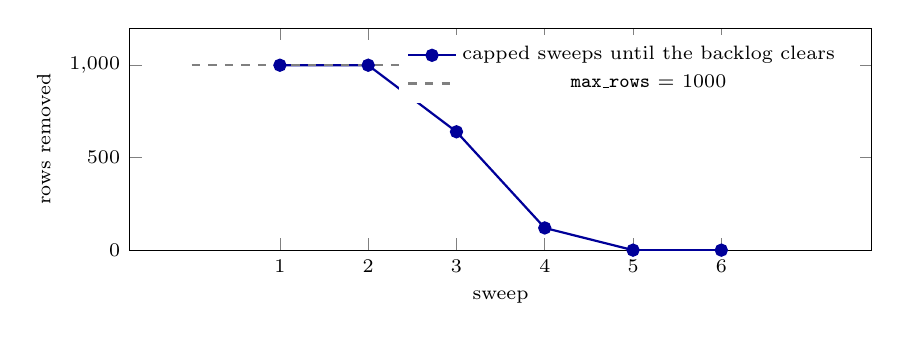
\begin{tikzpicture}
	\begin{axis}[
		width=11cm, height=4.4cm,
		xlabel={sweep}, ylabel={rows removed},
		ymin=0, ymax=1200,
		xtick={1,2,3,4,5,6},
		xlabel style={font=\scriptsize},
		ylabel style={font=\scriptsize},
		tick label style={font=\scriptsize},
		legend style={font=\scriptsize, draw=none},
		legend pos=north east,
	]
	\addplot[thick, mark=*, blue!60!black] coordinates {
		(1,1000) (2,1000) (3,640) (4,120) (5,0) (6,0)};
	\addlegendentry{capped sweeps until the backlog clears}
	\addplot[thick, dashed, gray, domain=0:7] {1000};
	\addlegendentry{\texttt{max\_rows} = 1000}
	\end{axis}
\end{tikzpicture}}
\captionof{figure}{The shape an operator should expect, illustrated, is several capped sweeps and
then quiet, while a store that reports 1\,000 on every sweep is receiving rows faster than the
policy expires them.}
\end{center}

\section{The queue store is a second store, with one writer}

The work queue is not a table in the run store. It is its own redb file with two tables ---
\texttt{queue\_item} keyed by item id and \texttt{queue\_event} keyed by \texttt{(id, seq)}
--- and a 4 MiB cache, in \texttt{crates/pii-store/src/queue.rs}. Keeping it separate means a
queue claim never competes for the write lock with a run's journal, and a store rebuilt for
one purpose does not have to be rebuilt for the other.

The single-writer rule shows up here in the protocol rather than in the process. The daemon is
the only writer; the CLI does not open the file. \texttt{pii queue add} sends a request over
the control socket, the engine's dispatch handles it, and the insertion and its
\texttt{queue.item.added} event are one transaction. A CLI that wrote the file directly would
be a second writer, and the daemon's in-memory view of the queue would be wrong until restart.

\begin{center}
\resizebox{\linewidth}{!}{%
\begin{tikzpicture}[node distance=8mm and 12mm]
	\node[b] (cli) {\texttt{pii queue add}};
	\node[b, right=of cli] (rpc) {socket request};
	\node[b, right=of rpc] (d) {daemon};
	\node[s, right=of d, yshift=8mm] (item) {queue\_item};
	\node[s, right=of d, yshift=-8mm] (ev) {queue\_event};
	\node[b, below=of d] (sched) {scheduler\\\scriptsize claim\_next};
	\node[b, right=of sched] (coder) {coder node};
	\node[b, below=of sched] (req) {requeue\_dead\_claims};

	\draw[f] (cli) -- (rpc);
	\draw[f] (rpc) -- (d);
	\draw[f] (d) -- (item);
	\draw[f] (d) -- (ev);
	\draw[f] (d) -- (sched);
	\draw[f] (sched) -- (coder);
	\draw[f] (req) -- node[p, right=2pt, midway]{dead claimant} (sched);
\end{tikzpicture}}
\captionof{figure}{One writer and one claim path, where the CLI reaches the store only through
the daemon and a claim is a status change plus its event in one transaction.}
\end{center}

\texttt{claim\_next} is the interesting method because it must be atomic against a second
caller. It opens one write transaction, reads every item, sorts by queue position, decides,
and --- only if the decision is a claim --- writes the item back as \texttt{Running} with its
attempt count incremented, its claimant recorded, and an \texttt{item.claimed} event appended,
all before the commit. A \texttt{Running} item short-circuits: the caller is told the queue is
already running something rather than being handed a second row.

\texttt{set\_status} follows the same shape: read the item, change its status, write it back,
journal \texttt{item.<status>} in the same transaction. That is what makes the queue's event
log sufficient to explain any row's state without reconstructing it from logs elsewhere.

\texttt{requeue\_dead\_claims} is the recovery path. It asks a caller-supplied predicate
whether the recorded claimant of a \texttt{Running} row is dead (an empty string for a row
with no recorded claim), returns those rows to \texttt{Pending}, and journals each as
\texttt{requeued\_after\_restart}. The returned count is what the daemon reports at boot. Two
properties matter: the predicate is supplied by the caller, so the store does not need to know
how to look up a process, and a row whose claimant is alive is left alone, so a second daemon
cannot steal work from a running one.

\begin{lstlisting}[language=bash]
pii queue add --id 376 --spec specs/376-retention-drops-what-the-policy-expires.md \
              --title "retention drops what the policy expires" \
              --criteria "cargo test -q -p pii-store --test retention_drops_what_the_policy_expires" \
              --touches crates/pii-store/src/retention.rs
pii queue ls
pii queue claim --by operator
\end{lstlisting}

\section{Bounded artefacts}

A store is one of several things a long-lived host fills. \texttt{pii disk} prints the others
in one table: the warm gate cache, the fresh-gate target, the coverage and tool target dirs,
the trash that parks work, and the gate exports outside the repository, each with bytes, age,
and \emph{the filesystem it sits on}. The filesystem column exists because a floor was once
measured on the wrong volume: two cleans freed 150 GB where nothing was short.

\begin{itemize}
	\item \texttt{\_tmp/gate-target} --- the warm build cache every gate step shares;
	\item \texttt{\_tmp/gate-target-fresh} --- the \texttt{--fresh} export's separate cache;
	\item \texttt{\_tmp/targets} --- per-step target dirs (clippy, doctest, tools);
	\item \texttt{\_tmp/\_trash} --- in-repo quarantined work;
	\item \texttt{/projects/\_tmp} --- \texttt{fresh-gate-<pid>} exports;
	\item \texttt{/projects/\_trash} --- quarantined working trees, one directory per park;
	\item \texttt{/tmp/\_trash-podman} --- container scratch that outlives a run;
	\item \texttt{/tmp/gate-cache} --- tool caches outside the repository.
\end{itemize}

Each row carries bytes, age and the owning filesystem, because the question an operator asks
is not ``how big is this'' but ``which volume is short''.

Each has an owner and a ceiling. The warm cache is capped at 40 GiB by
\texttt{FRESH\_GATE\_CACHE\_MAX\_GB}, and is trimmed before a build only when no cargo or
rustc is live --- a running build would lose its target under it. The trajectory directory is
bounded by bytes and file count (512 MiB and 50\,000 by default) and prunes the oldest
finished runs. The store's own page cache is 8 MiB, which is the subject of the next section.

\section{The two numbers that were wrong}

\paragraph{The page cache.} redb defaults to a 1 GiB cache. For a control-plane daemon holding
a store of a few megabytes that is not a tuning detail; under soak it appeared as a slow,
sublinear RSS climb with a flat thread count, a flat descriptor count, and a store file of a
few megabytes. The climb was in no code that owned a connection or a thread. Setting the cache
to 8 MiB left ample headroom under the 50 MB budget the RSS gate enforces.

\paragraph{The index nothing read.} \texttt{RESUME\_INDEX} was declared in \texttt{tables.rs},
opened three times in \texttt{lib.rs}, written by the scheduler's dispatch path, and counted
into the identity stats. The code's own comment at the write site said that nothing read it.
The cost was real --- an index write on every resume --- and the number invited an operator to
trust a structure with no reader. Spec 375 removed the table, every \texttt{open\_table}, the
write site, and the stat, while explicitly keeping \texttt{RUN\_JOURNAL} and
\texttt{RUN\_BY\_STATUS}, which are read. The guardrail in that spec is the useful part for a
reviewer: do not drop a table because it looks unused; drop it because you found the reader
that does not exist.

\section{Format version and identity}

A store records a format version in \texttt{meta}. Opening a store whose recorded version is
\emph{newer} than the binary understands is refused with both numbers in the message, so an
old binary never writes into a layout it does not know. A fresh or pre-versioning store is
stamped on open. The auxiliary stores --- approvals, heal, memory, channel, timer, queue ---
are stamped the same way through one shared function, so there is one rule and not six.

\texttt{Store::info} reports the path, the file size, the format version, the last write time,
and per-table entry counts. It counts six tables, not all of them: \texttt{graph\_body},
\texttt{run}, \texttt{run\_journal}, \texttt{run\_snapshot}, \texttt{session},
\texttt{session\_msg}. That is a deliberate short list --- the counts an operator needs to
answer ``is this store growing, and in which of the two big things'' --- and \texttt{pii store
stats} surfaces it. The health record carries the same numbers under \texttt{entries.<table>},
so a probe can compare two hosts without reading either store.

\begin{lstlisting}[language=bash]
pii store stats
pii store compact      # daemon stopped
pii store prune        # daemon stopped
\end{lstlisting}

\section{What a single run writes}

A worked example makes the accounting concrete. One run of a four-node graph, with two node
calls, writes the following (an illustrative count, not a captured run):

\begin{itemize}
	\item one row in \texttt{run} (rewritten on every append, so the header is the hot row);
	\item one \texttt{run\_journal} row per event: started, node started, node finished, node
	started, node finished, finished --- six rows for four nodes, because the run itself emits
	two;
	\item one \texttt{run\_by\_status} entry, rewritten as the status moves, and removed from
	the old status bucket each time;
	\item one \texttt{sys\_status\_run} row and one rewrite of the \texttt{sys\_status} totals;
	\item zero \texttt{graph\_body} rows on the second and later runs of the same graph,
	because the body is already stored under its hash.
\end{itemize}

The header being hot is why the append path rewrites it once per call rather than once per
event: batching events into one append is what keeps a chatty node from paying a header write
per event.

\section{Failure modes worth recognising}

\begin{enumerate}
	\item \textbf{A second writer.} Two processes on one store interleave writes or refuse; the
	symptom is a lock error naming the file, usually from a test that inherited the operator's
	\texttt{PII\_STATE\_DIR}. The fix is that every test daemon owns its own state directory.
	\item \textbf{A counter that lags.} A health number that changes only after a restart means
	the observer is installed after the first writes, or is not installed at all. The rebuild
	walk is how to tell lag from corruption.
	\item \textbf{A sweep that deletes what it cannot date.} Symptom: a store that loses its
	oldest and most interesting runs first, and a fixture that fails only with seeded pre-clock
	rows.
	\item \textbf{A sweep that blocks.} Symptom: every append stalls for the duration of one
	sweep. The cap is the fix, and a sweep that reports exactly 1\,000 is the evidence that it
	is working.
	\item \textbf{A table with no reader.} Symptom: a statistic nobody can act on, and a write
	cost on a hot path. The test is to delete the table and see whether any test fails for the
	right reason.
	\item \textbf{A cache that grows toward its default.} Symptom: RSS climbing with flat
	threads and flat descriptors, no leak in any owner. Check the embedded database's cache
	before rewriting the connection pool.
\end{enumerate}

Each of these was observed here, and each is now pinned by a test that fails if the fix is
reverted: the transaction count for id blocks, the transaction count for a duplicate graph
body, the undateable-row fixture, the live-run fixture, and the identity report.
